\section{Mechanism Design}

\subsection{Initiatives, not Proposals}
\signals{} works with \emph{Initiatives}---ideas or actions seeking support. Initiatives live inside Boards (configuration sets), and DAOs can run multiple Boards with different parameters. Board configs are on-chain, so DAOs can govern them directly.

\subsection{Token-Locking}
Participants lock existing tokens for a chosen duration to express commitment; locking against an Initiative is not supported. Each lockup mints a transferable NFT bond redeemable when the lock expires, enabling secondary markets or other reputation measures. Boards typically use governance tokens but can target any ERC-20.

\subsection{Calculating Support}
Time is measured in Epochs (Board-defined). Longer locks provide more weight:
\begin{equation}
  S = T \times D^{k}
\end{equation}
where $S$ is support, $T$ is tokens locked, $D$ is duration in Epochs, and $k$ is an exponential bonus favoring longer commitments. Tuning $k$ prevents short, large locks from dominating and lets smaller holders compete by committing longer.

\begin{figure}[h]
  \centering
  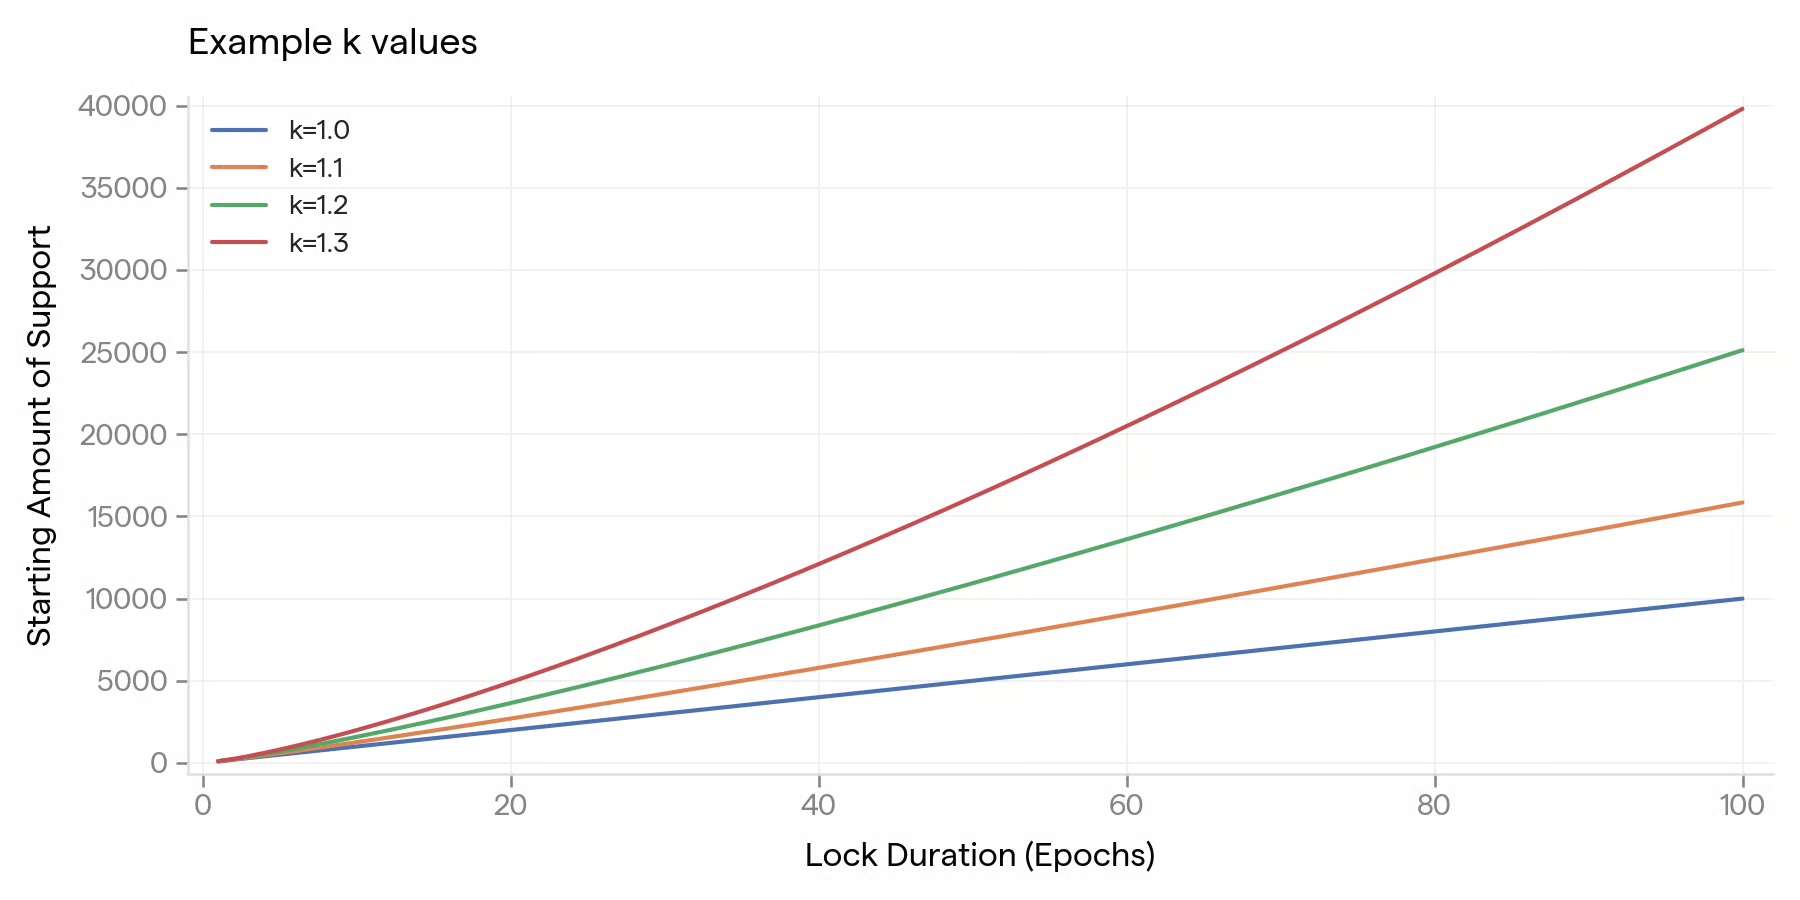
\includegraphics[width=0.85\linewidth]{figures/fig-boost-lockup.png}
  \caption{Adjusting $k$ changes how much additional weight longer lockups receive.}
\end{figure}

\subsection{Decay}
Support decays over time to keep rankings current. Each Board specifies a decay curve (linear, exponential, or custom). Current support for Initiative $i$ at time $t$ sums decayed contributions from its locks $\ell$:
\begin{equation}
  \text{CurrentSupport}_i(t) = \sum_{\ell \in \text{Locks}_i} \text{Weight}(\ell, t).
\end{equation}
Decay ensures abandoned initiatives fade, early interest provides a head start (not permanence), and manipulation via stale locks is limited.

\subsection{Actioning Initiatives}
Boards define an acceptance threshold. When current support exceeds it, an Initiative can be actioned: the Initiative closes and all supporting tokens unlock early. DAOs decide whether actioning is automatic or requires a trigger (committee, vote, or other mechanism). The early unlock incentivizes backing only initiatives expected to succeed.

\subsection{Examples of Support and Thresholds}
\begin{figure}[h]
  \centering
  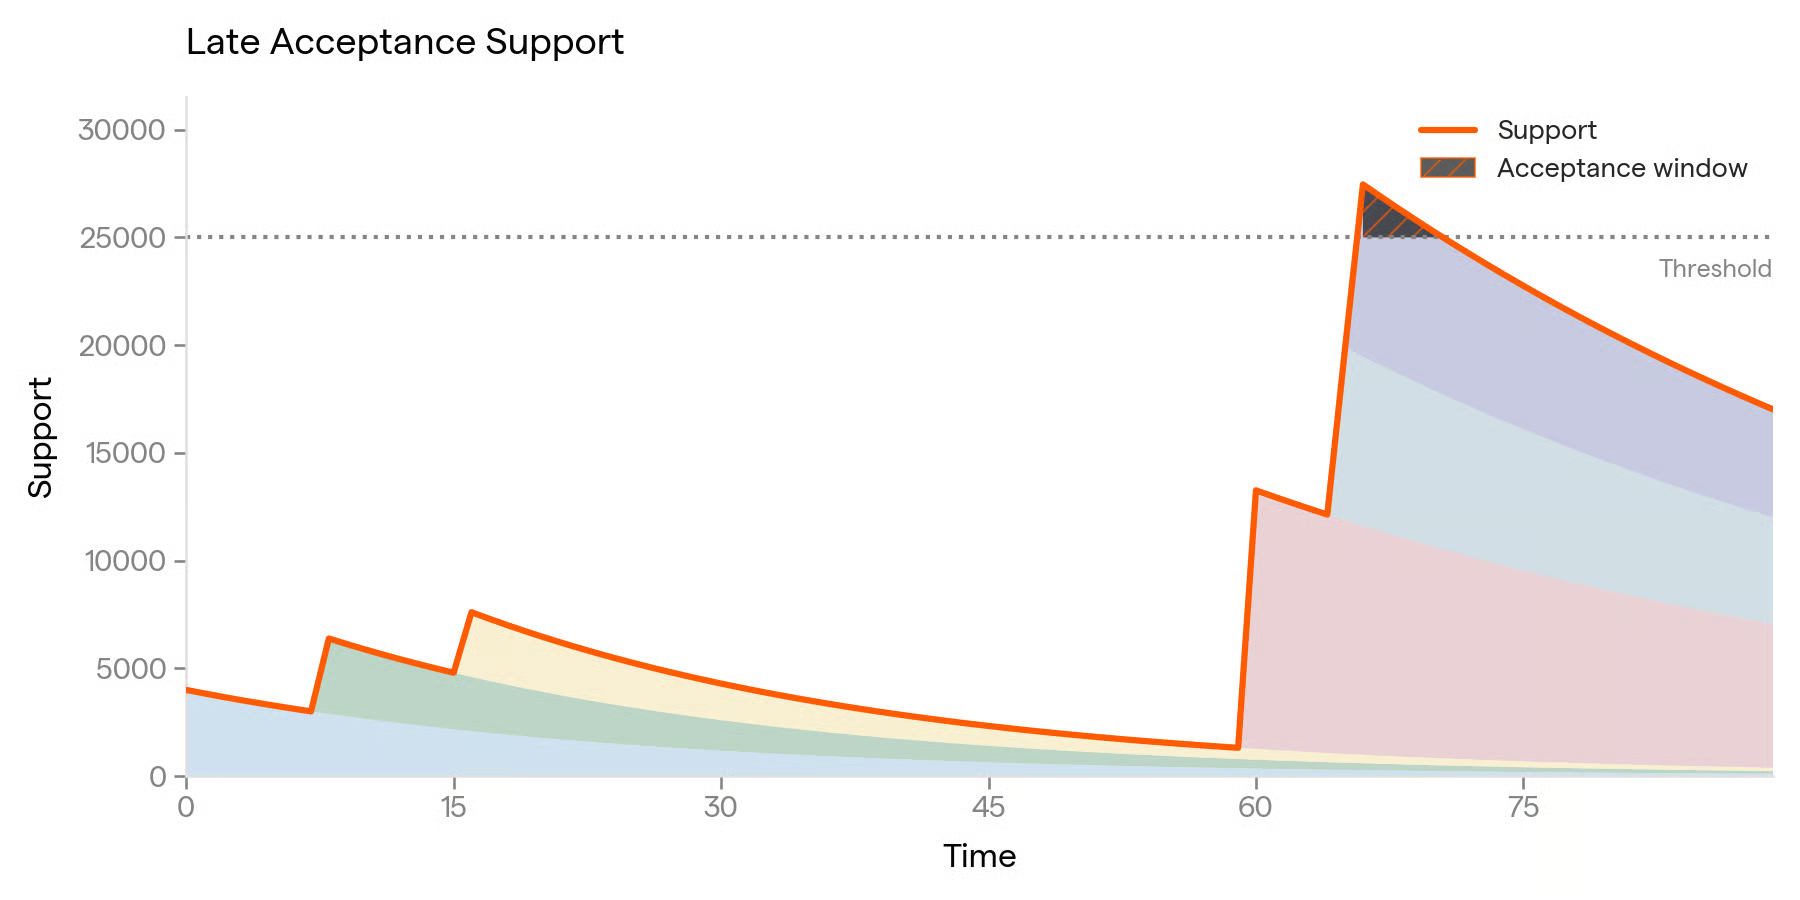
\includegraphics[width=0.85\linewidth]{figures/fig-late-acceptance.png}
  \caption{Early support is insufficient; renewed interest later can re-open the path to action.}
\end{figure}

\begin{figure}[h]
  \centering
  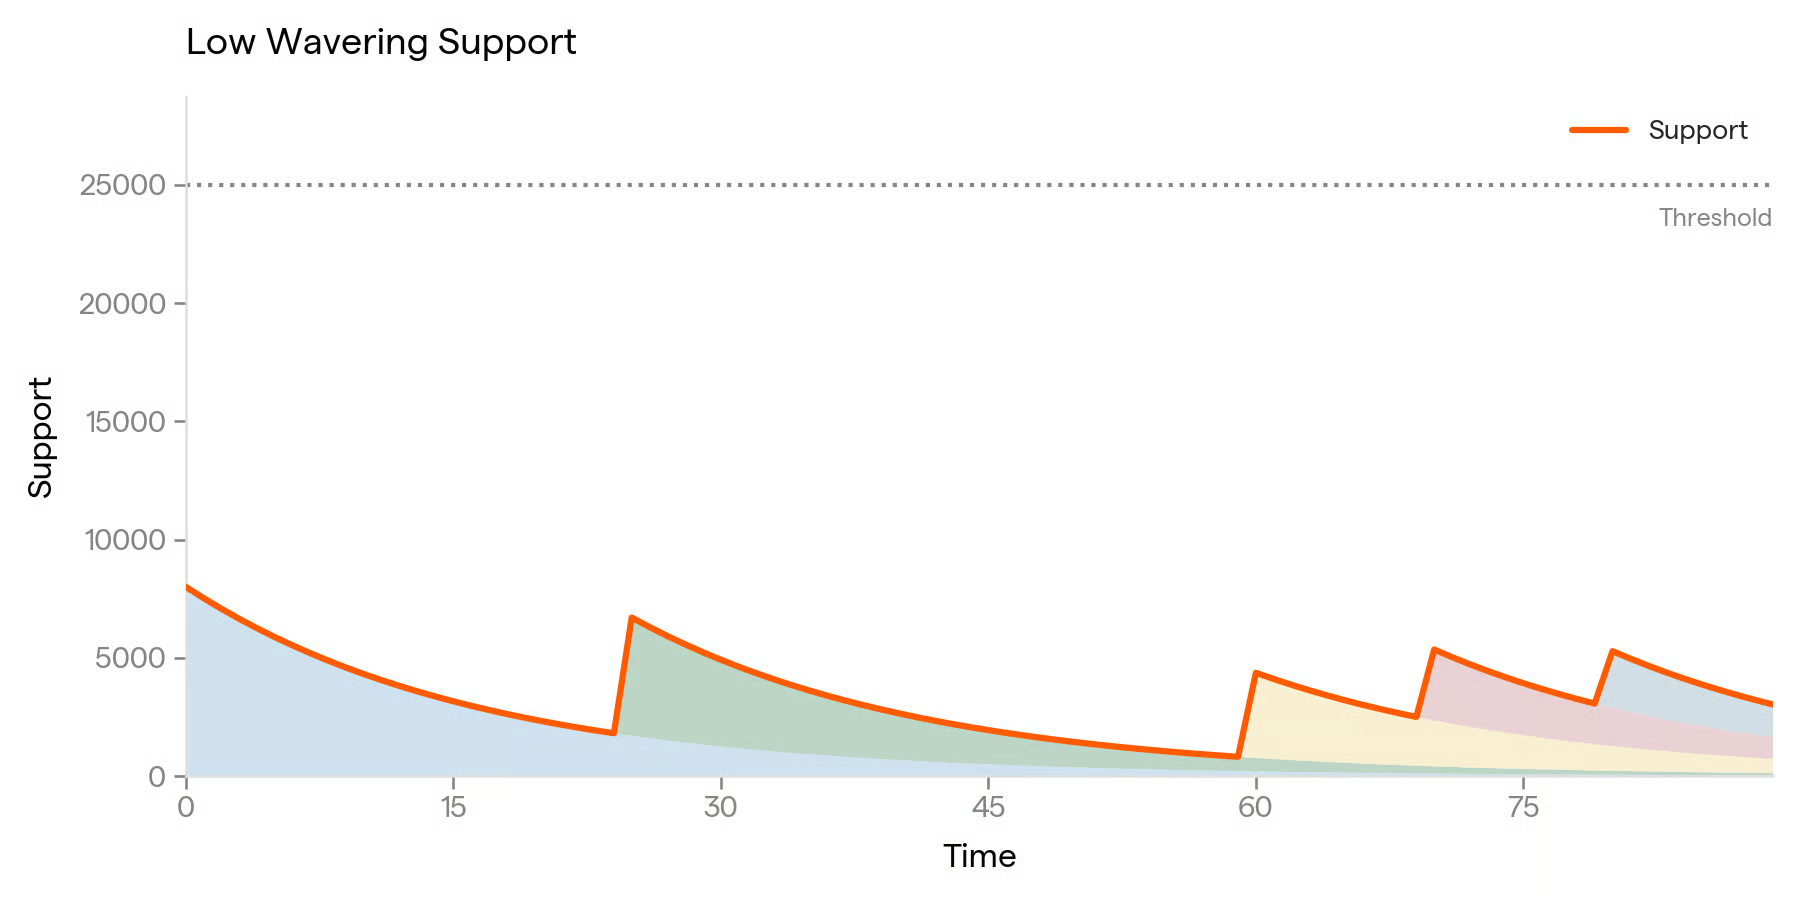
\includegraphics[width=0.85\linewidth]{figures/fig-low-wavering-support.png}
  \caption{Insufficient, wavering support never crosses the threshold despite cumulative effort.}
\end{figure}

\begin{figure}[h]
  \centering
  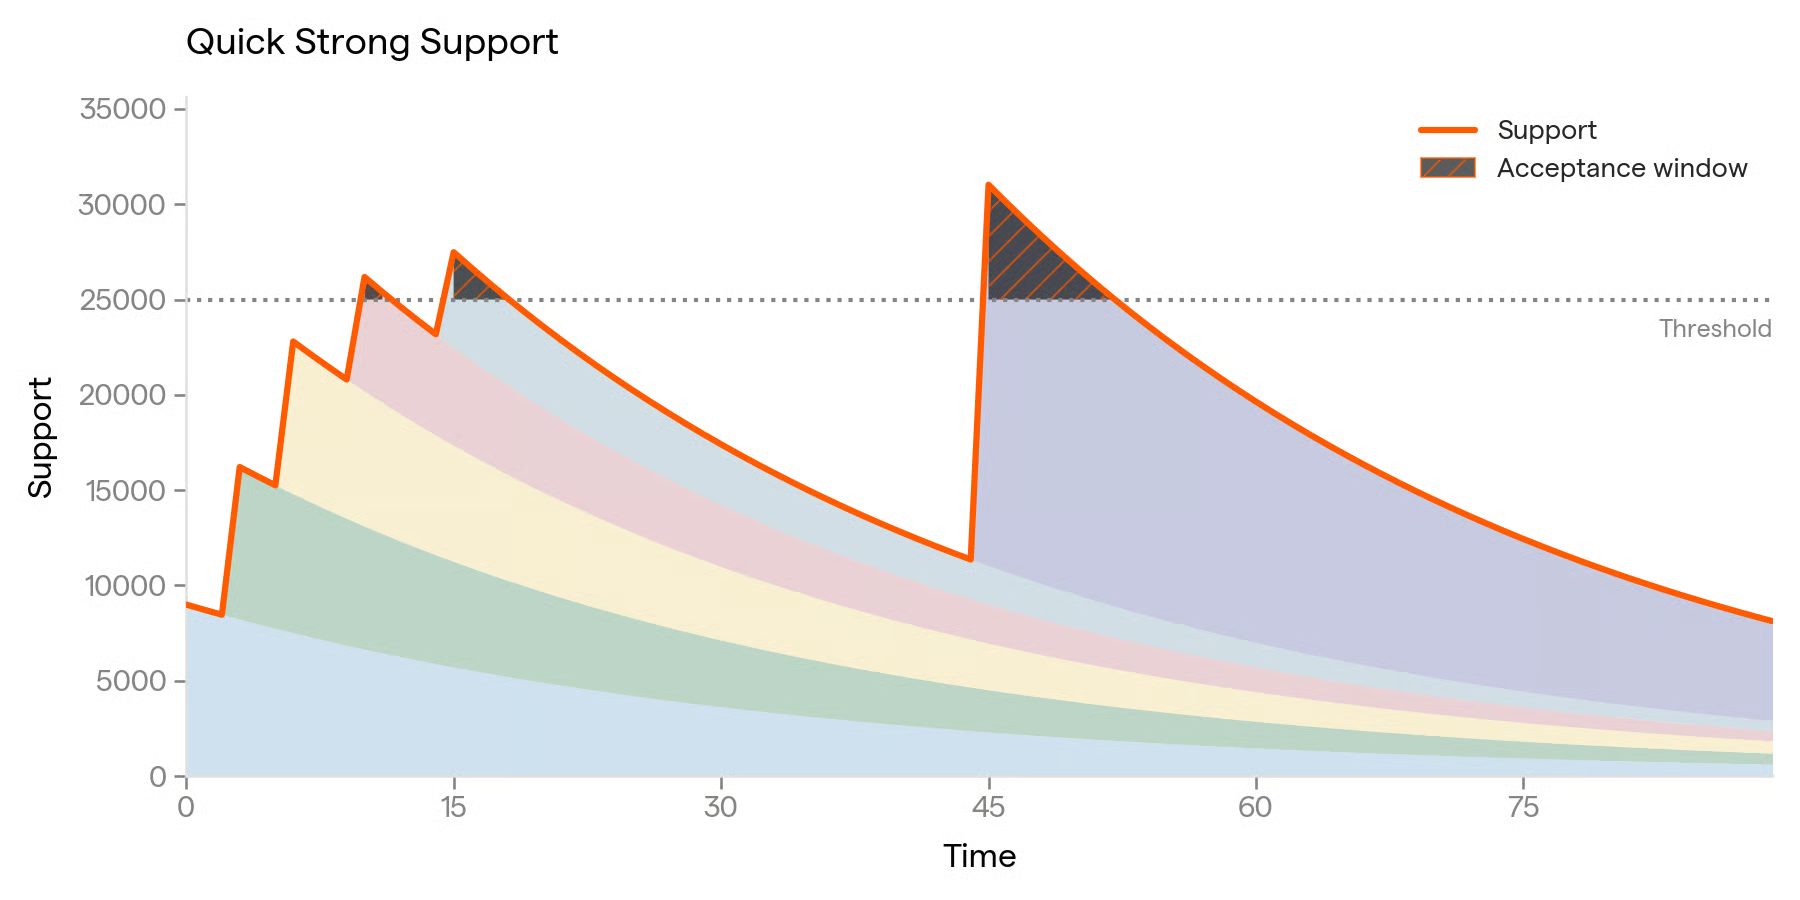
\includegraphics[width=0.85\linewidth]{figures/fig-quick-support.png}
  \caption{Late momentum pushes an Initiative over the threshold after an initial lull.}
\end{figure}

\subsection{Endorsements (Optional)}
If a DAO uses delegated voting, delegates may not own the tokens they wield. Boards can optionally require binary \emph{Endorsements} tied to delegated voting power in addition to lockups. Caps on endorsements per Initiative encourage delegates to act early and visibly.
